\documentclass[12pt,a4paper]{amsart}
\usepackage[UTF8]{ctex}
\usepackage{preamble}


\title{阻尼振动和受迫振动物理实验}

\begin{document}

\maketitle

\section{实验目的}

\begin{enumerate}
    \item 通过实验,学习测量振动系统基本参数的方法;
    \item 研究受迫振动的幅频特性和相频特性,观察共振现象;
    \item 观测不同阻尼对受迫振动的影响。
\end{enumerate}

\section{实验仪器}

本实验所用仪器是专门研究振动的波耳共振仪,仪器结构如 \ref{fig:instruments} 所示。

\begin{figure}[H]
    \centering
    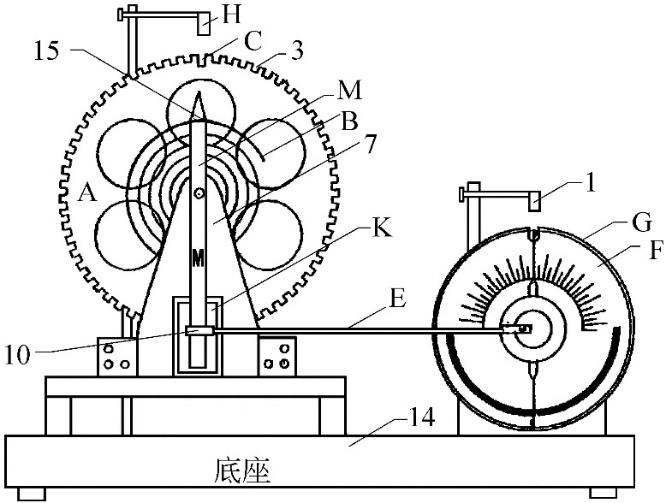
\includegraphics[width=0.5\textwidth]{img/instruments.jpg}
    \caption{波耳共振仪结构示意图}
    \label{fig:instruments}
\end{figure}

铜质圆形摆轮 A 与弹簧 B 构成待测的振动系统,弹簧 B 的另一端固定在摇杆 M 上的点 15 的位置处。摆轮边沿有一圈周期为 $2^\circ$ 的槽形缺口,光电门 H 通过测定缺口移动的个数来记录振动的幅度,其中有一长缺口 C 是平衡位置的标志,是测量摆轮振动周期的参考点,也是控制闪光灯开关以测量受迫振动与外激励之间的相位差的参考点。

外激励是由转速极为稳定且可调的电机的偏心轴通过连杆 E 和摇杆 M 加到振动系统上。由于连杆 E 较长,电机匀速转动时对系统的作用可看作简谐激励,改变电机转速就改变了外激励的周期。带有标志电机位置刻线(0 位标志线)的有机玻璃转盘 F 同电机一同转动。

当摆轮 A 的长缺口 C 通过平衡位置时,闪光灯点亮,照亮有机玻璃盘 F 的 0 位标志线,此刻 0 位标志线指示的角度即为外激励超前摆轮振动的角度,亦即摆轮滞后于外激励的角度。

闪光灯在长缺口 C 来回通过光电门 H 时都要闪亮,因此每周期闪亮两次。在摆轮完全不受外激励作用且光电门 H 正好处于平衡位置时,闪光灯照亮 0 位标志线的两次示值应完全一致,但由于整体结构的一致性差,这一点并不能处处保证。实际上两次角度示值可能有少许偏差,我们可取其平均值作为被测的角度。

由阻尼线圈 K 产生电磁阻尼作用于摆轮。调整线圈电流可改变电磁铁气隙中磁场,从而改变阻尼力矩。阻尼选择旋钮置 0 时,线圈中无电流,是最小阻尼的状态。调节阻尼选择旋钮,能改变线圈中的电流,也就改变了阻尼。由于线圈用直流励磁,可能因材料中的剩磁或磁滞现象而使阻尼状态与旋钮位置不呈单值对应关系,因此在做某一阻尼状态的实验测量过程中不可改变阻尼状态,直至该阻尼状态的实验完全做完。

\section{实验原理}

\subsection{有粘滞阻尼的阻尼振动}

对于弹簧与摆轮组成的振动系统(如图1所示),设摆轮转动惯量为$J$,粘滞阻尼的阻尼力矩大小定义为角速度$\frac{d\theta}{dt}$与阻尼力矩系数$\gamma$的乘积,弹簧劲度系数为$k$,弹簧的反抗力矩为$-k\theta$。忽略弹簧的等效转动惯量,则转角$\theta$的运动方程为

\begin{equation}
    J\frac{d^2\theta}{dt^2} + \gamma\frac{d\theta}{dt} + k\theta = 0 \label{eq:1}
\end{equation}

记 $\omega_0$ 为无阻尼时自由振动的固有角频率,其值为 $\omega_0 = \sqrt{\frac{k}{J}}$,定义阻尼系数 $\beta$ 为 $\beta = \frac{\gamma}{2J}$ ,则 \ref{eq:1} 变为

\begin{equation}
    J\frac{d^2\theta}{dt^2} + 2\beta\omega_0\frac{d\theta}{dt} + \omega_0^2\theta = 0 \label{eq:2}
\end{equation}

对于弱阻尼即 $2\beta\omega_0 \ll 1$ 的情况,阻尼振动运动方程 \ref{eq:1} 的解为

\begin{equation}
    \theta = \theta_i e^{-\beta t}\cos(\omega t + \phi) \label{eq:3}
\end{equation}

式中 $\theta_i$ 为摆幅,$\phi$ 为初始相位。由上式可知,阻尼振动角频率为 $\omega = \sqrt{\omega_0^2 - \beta^2}$,相应的阻尼振动周期为 $T = \frac{2\pi}{\sqrt{\omega_0^2 - \beta^2}}$。

\begin{figure}
    \centering
    \begin{subfigure}[b]{0.2475\linewidth}
        \centering
        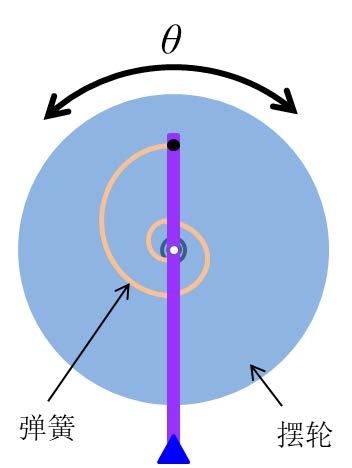
\includegraphics[width=\linewidth]{img/1.jpg}
        \caption{弹簧与摆轮}
        \label{fig:1}
    \end{subfigure}
    \hfill
    \begin{subfigure}[b]{0.2475\linewidth}
        \centering
        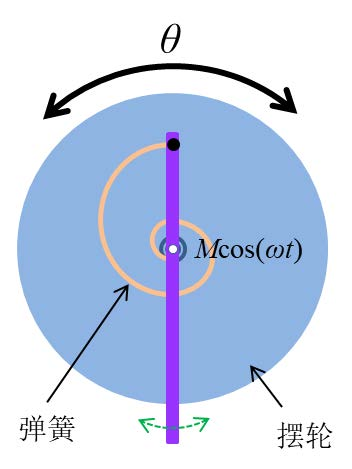
\includegraphics[width=\linewidth]{img/2.jpg}
        \caption{周期外力矩}
        \label{fig:2}
    \end{subfigure}
    \hfill
    \begin{subfigure}[b]{0.405\linewidth}
        \centering
        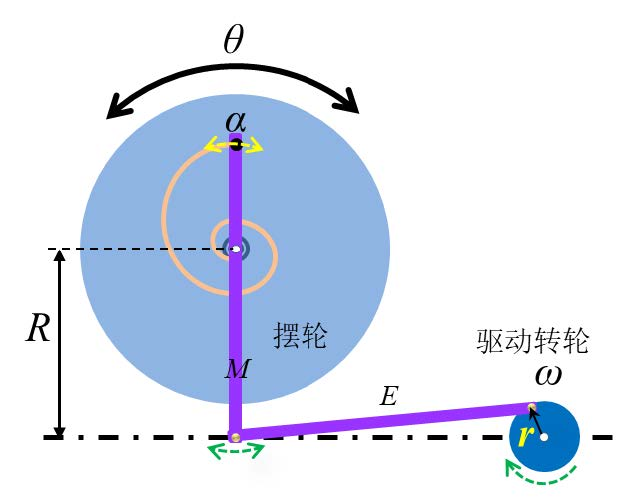
\includegraphics[width=\linewidth]{img/3.jpg}
        \caption{波耳共振仪转轮驱动示意图}
        \label{fig:3}
    \end{subfigure}
\end{figure}

\subsection{周期外力矩作用下的受迫振动}

在周期外力矩 $\cos(Mt\omega)$ 激励下(见图 \ref{fig:2})的运动方程和方程的通解分别为:

\begin{equation}
    J\frac{d^2\theta}{dt^2} + \gamma\frac{d\theta}{dt} + k\theta = \omega^2 \cos(Mt\omega) \label{eq:4}
\end{equation}

\begin{equation}
    \theta = \frac{2}{m}\left(0 e^{-\beta t}\cos(\omega t - \phi) + i e^{-\beta t}\sin(\omega t - \phi) + \frac{M}{k}\cos(Mt\omega) - \frac{\gamma}{2m}\omega t + \frac{\gamma M}{2k}\sin(Mt\omega)\right) \label{eq:5}
\end{equation}

通解 \ref{eq:5} 是形如式 \ref{3} 的阻尼振动和频率同激励源频率的简谐振动的叠加。阻尼振动项反映一定初始条件后的过渡过程,$t \rightarrow \infty$ 则该项为 0。一般 $t \gg \tau$ 之后($\tau$ 为阻尼振动振幅衰减到 $e^{-1}$ 即36.8\% 时所用的时间),就有稳态解:

\begin{equation}
    \theta_m \cos(\omega t - \phi) \label{eq:6}
\end{equation}

稳态解的振幅和相位差分别为:

\begin{equation}
    \theta_m^2 = \frac{2M}{J\omega^2} - \frac{\gamma^2}{4m\omega^2} \label{eq:7}
\end{equation}

\begin{equation}
    \phi = \arctan\left(\frac{\beta}{\omega}\right) - \arctan\left(\frac{\gamma}{2m\omega}\right) \label{eq:8}
\end{equation}

式 \ref{eq:8} 中相位差 $\phi$ 的取值范围为 $0 < \phi < \pi$,反映摆轮振动总是滞后于激励源支座的振动。

\subsection{转轮驱动下的受迫振动运动方程及解}

利用转轮连杆结构对摆盘施加周期性驱动力矩,如图3所示波耳共振仪驱动原理。当连杆E的长度和
摇杆M的长度远大于连杆在转轮上的连接点到转轮轴心的距离$r$时,若驱动转轮的以角速度$\omega$匀速旋转,可以证明,系统调节对称后,弹簧支座(摇杆M上与弹簧的连接处)的偏转角的一阶近似式可以写成:

\begin{equation}
    \alpha = \alpha_m \cos(\omega t) = \alpha \omega \tag{9}
\end{equation}

$\alpha_m$是摇杆摆幅,$R$是图3中连杆E与摇杆M的接点到摇杆和摆轮共同的转轴中心的距离。由于弹簧的支座在运动,运动支座是激励源。弹簧总转角为 $\cos(\theta_m - \alpha t) = \theta - \alpha \omega t$,仿照式(4),在固定坐标系中摆轮转角$\theta$的运动方程为:

\begin{equation}
    J\frac{d^2\theta}{dt^2} + \gamma\frac{d\theta}{dt} + k\theta - \alpha \omega = 0 \tag{10}
\end{equation}

上式可以改写成:

\begin{equation}
    J\frac{d^2\theta}{dt^2} + \gamma\frac{d\theta}{dt} + k\theta = \alpha \omega \tag{4'}
\end{equation}

该式和弹簧支座固定、摆轮受周期外力矩$M\cos(\omega t)$作用时的运动方程在形式上完全一致,等效外激励力矩的振幅为$k\alpha_m$。方程(4')的通解与稳态解的形式分别同(5)和(6)式;这表明图3的装置是一个十分巧妙的设计,得到了与周期外力矩作用下相同形式的解。(这和一般文献描述的常用的支座周期运动激励的方程不同,因一般情况下粘滞阻尼力矩正比于以支座方位为极坐标极轴的角速度,而实验用波耳共振仪中电磁阻尼线圈$K_{2024}$春物理实验A(1)课程资料——28——是固定不动的,参见图5)。稳态解的相位差表达式仍为式(8),而式(7)变为:

\begin{equation}
    \theta_m^2 = \frac{2\alpha}{\omega^2} - \frac{\gamma^2}{4m\omega^2} \tag{7'}
\end{equation}

由$\theta_m$的极大值条件$0 = \frac{\partial \theta}{\partial \omega}$ 可知,当外激励角频率$2\omega = \omega_0^2 - \beta^2$时,系统发生共振,$\theta_m$有极大值,其值为:

\begin{equation}
    \theta_m = \frac{2\alpha}{\omega_0^2 - \beta^2}
\end{equation}

引入参数$\zeta = \frac{\beta}{\omega_0} = \frac{\gamma}{2\sqrt{kJ}}$,称为阻尼比。振幅$\theta_m$和相位差$\phi$是支座振幅$\alpha_m$、阻尼比$\zeta$和频率比$\frac{\omega}{\omega_0}$的函数(自己推导),它们随频率比变化的曲线分别叫做幅频特性曲线和相频特性曲线(参见图4)。测定并分析这些曲线,有助于对受迫振动规律的深入理解。

\subsection{描述阻尼振动的常用参量}

\textbf{表1 方程中参量与符号}

\begin{center}
    \begin{tabular}{|c|c|}
        \hline
        方程中的参量 & 符号                            \\
        \hline
        转动惯量     & $J$                             \\
        劲度系数     & $k$                             \\
        阻尼力矩系数 & $\gamma$                        \\
        固有角频率   & $\omega_0 = \sqrt{\frac{k}{J}}$ \\
        外激励角频率 & $\omega$                        \\
        \hline
    \end{tabular}
\end{center}

\textbf{表2 文献中描述阻尼振动的常用参量及其计算公式}

\begin{center}
    \begin{tabular}{|c|c|p{6cm}|}
        \hline
        名称            & 符号及公式                                                             & 定义或说明                                                                                                                              \\
        \hline
        1. 阻尼系数     & $\beta = \gamma (2J)$                                                  & 标准定义,但机械、力学文献中常用上表中的 $\gamma$。                                                                                     \\
        2. 阻尼比       & $\zeta = \frac{\gamma}{2 \sqrt{kJ}} = \frac{\beta}{\omega}$            & damping ratio,无量纲。                                                                                                                 \\
        3. 阻尼振动周期 & $T = \frac{2\pi}{\omega - \beta}$ 或 $\frac{2\pi}{\sqrt{1 - \zeta^2}}$ &                                                                                                                                         \\
        4. 时间常数     & $\tau = \frac{2J}{\gamma} = \frac{1}{\beta}$                           & time constant,阻尼振动的振幅衰减到原来的1/e的时间,单位为s(秒)。                                                                     \\
        5. 品质因数     & $Q = \frac{1}{2\zeta}$                                                 & (机械振动系统中的定义)系统共振锐度或频率选择性的量度。一般定义为系统储能 $E$ 与周期能耗 $\Delta E$ 之比($E/\Delta E$)的 $2\pi$ 倍。 \\
        6. 对数减缩率   & $\Lambda = \frac{1}{T\tau} = \pi(\zeta - \zeta)$                       & 定义为衰减阻尼振动中相邻两循环的振幅比的自然对数。                                                                                      \\
        \hline
    \end{tabular}
\end{center}

\section{实验内容}

\subsection{调整仪器使波耳共振仪处于工作状态}
\begin{enumerate}
    \item 关断电机和闪光灯开关,打开电源开关,阻尼开关置于0档。
    \item 手动微调光电门H、I,避免与摆轮或相位差测量盘接触。
    \item 手动调整电机偏心轮使有机玻璃转盘F上的0位标志刻线指示0度,即通过连杆E和摇杆M使摆轮处于平衡位置。
    \item 拨动摆轮使其偏离平衡位置约120°~150°,松开手后,检查摆轮的自由摆动情况。正常情况下,振动衰减应该很慢。
\end{enumerate}

\subsection{测量最小阻尼条件下系统的阻尼比$\zeta$和固有角频率$\omega_0$}
\begin{enumerate}
    \item 光电门选择开关置于“摆轮”位置,拨动摆轮使其偏离平衡位置约120°~150°后松手,摆轮开始摆动。
    \item 由大到小依次读取显示窗中的振幅值$\theta_1$,$\theta_2$,$\theta_3$,$\dots$,$\theta_j$,$\dots$,$\theta_n$;周期选择开关选择“10”,按复位钮启动周期测量,停止时读取所显示的时间$T_d$。
    \item 计算阻尼比$\zeta$及其不确定度$\Delta\zeta$,以及固有角频率$\omega_0$及其不确定度$\Delta\omega_0$。
\end{enumerate}

\subsection{测量较强阻尼条件下的阻尼比$\zeta$}
选择其它2种阻尼挡位(2、3档位或2、4档位),类似上述的方法测量较强阻尼条件下的阻尼比$\zeta$。

\subsection{测定受迫振动的幅频特性和相频特性曲线}
选择2个不同阻尼比的阻尼档位(与任务3中的档位选择保持一致),测量摆轮做受迫振动的幅频特性和相频特性曲线。

\section{数据处理及结果}
\section{实验小结}

\begin{enumerate}
    \item 为避免剩磁影响,阻尼开关不要随便拨动;
    \item 只有测受迫振动相频特性时才开启仪器面板上的闪光灯开关,读完数据后迅即关闭;
    \item 相频特性与幅频特性测量要在振动稳定后进行,可根据测量数据计算 $\tau$ 值和达到稳定态($e^{-t/\tau}<0.01$)所需要的时间;
    \item 在共振点附近要注意随时调节$\omega$,勿使振幅过大($\theta_{\text{max}}<180^\circ$)以免损坏波耳共振仪,在阻尼较小时尤其要小心操作;
    \item 几种阻尼状态下的幅频特性曲线和相频特性曲线要画在同一张坐标纸上,以便进行比较。
\end{enumerate}

\section{原始数据记录}

% \cite{Abu-Zurayk2013}\cite{Gerritsma2008}\cite{Gerritsma2008}\cite{Baseski2014}

\appendix


\bibliographystyle{unsrt}
{\footnotesize\bibliography{./library}}


\end{document}
